\chapter{Magnetostatik}

\textbf{Elektrostatik:}\\
ruhende Ladungen $ \Rightarrow $ es wirken Zeitunabhängige elektrische Felder $ \vec{E}(\vec{r}) $\\[5pt]
\textbf{Magnetostatik:}\\
magnetische Felder entstehen aus \textbf{bewegten Ladungen}\\
Kraft auf bewegte Ladung:
\begin{equation*}
\vec{F} = q (\vec{E} + \vec{v} \times \vec{B})
\end{equation*}
\lcom{Magnetfelder von Bewegten Ladungen sind zeitlich verändert und daher kompliziert zu beschreiben. Daher verwenden wir hier ersteinmal statische Ströme die konstande Magnetfelder erzeugen.}\\[3pt]
Magnetostatik:
$$ \begin{array}{c}
\tx{stationäre}\\ \tx{Ströme}
\end{array} \Rightarrow \begin{array}{c}
\tx{zeitunabhängige} \\ \tx{Magnetfelder} \\ \vec{B}(\vec{r})
\end{array} $$
\lcom{Zunächst müssen wir erst einige Dinge Definieren:}

\section{Strom, Stromdichte und Kontinuitätsgleichung}

\subsection{Strom}

\begin{minipage}{.6\linewidth}
	metallischer Leiter:
	\begin{equation*}
	I = \frac{\tx{Ladung}}{\tx{Zeit}} = \frac{\Delta q}{\Delta t} \qquad [I] = 1 \, \tx{A} = \tx{C s}^{-1}
	\end{equation*}
\end{minipage}%
\begin{minipage}{.4\linewidth}
	\centering
	%t4:
	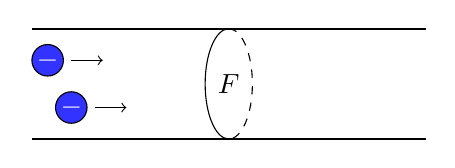
\begin{tikzpicture}
		\draw[-,thick] (-2,.7) -- (3,.7);
		\draw[-,thick] (-2,-.7) -- (3,-.7);
		\draw (.5,.7) arc[start angle=90,end angle=270, x radius=0.3, y radius=.7];
		\draw[dashed] (.5,0.7) arc[start angle=90,end angle=-90, x radius=0.3, y radius=.7] node[yshift=.7cm] {$F$};
		\draw[fill = white!20!blue] (-1.8,.3) circle (.2cm) node[] {$ \color{white} - \color{white} $};
		\draw[fill = white!20!blue] (-1.5,-.3) circle (.2cm) node[] {$ \color{white} - \color{white} $};
		\draw[->] (-1.5,.3) -- (-1.1,.3);
		\draw[->] (-1.2,-.3) -- (-.8,-.3);
	\end{tikzpicture}
	\vspace{5pt}
\end{minipage}%
\\[10pt]
\emph{Beispiel:} \textbf{Stationärer Strom}\\[5pt]
\begin{minipage}{.6\linewidth}
	Ladungsträger mit:\\
	$ v : $ Geschwindigkeit ($ \const $)\\
	$ n : $ homogene Dichte\\
	$ q : $ Ladung
\end{minipage}%
\begin{minipage}{.4\linewidth}
	%t5:
	\centering
	\begin{tikzpicture}
		\draw[dashed] (-2,.7) arc[start angle=90,end angle=-90, x radius=0.3, y radius=.7];
		\draw[pattern = north east lines,pattern color = black!30!white] (-2,.7) -- (.5,.7) arc[start angle=90, end angle=270, x radius=.3, y radius=.7] -- (-2,-.7) arc[start angle=270, end angle=90, x radius=.3, y radius=.7];
		\draw[draw=none, fill = black!10!white] (.5,0) ellipse (0.3cm and 0.7cm);
		\draw[-,thick] (-3,.7) -- (2,.7);
		\draw[-,thick] (-3,-.7) -- (2,-.7);
		\draw (.5,.7) arc[start angle=90,end angle=270, x radius=0.3, y radius=.7];
		\draw[dashed] (.5,0.7) arc[start angle=90,end angle=-90, x radius=0.3, y radius=.7] node[yshift=.7cm] {$F$};
		\draw[fill = white!20!blue] (-1.8,.3) circle (.2cm) node[] {$ \color{white} - \color{white} $};
		\draw[fill = white!20!blue] (-1.5,-.3) circle (.2cm) node[] {$ \color{white} - \color{white} $};
		\draw[->] (-1.5,.3) -- (-1.1,.3);
		\draw[->] (-1.2,-.3) -- (-.8,-.3);
		\draw[decorate, decoration={brace,amplitude=10pt,mirror,raise=2pt}]  (-2,-.7) -- node[below=12pt] {$\Delta x = v \Delta t$}  (.5,-.7);
	\end{tikzpicture}
\end{minipage}%
\\
Leiter mit:
$ F : $ Querschnittsfläche\\[5pt]
in $ \Delta t : \quad n \cdot F \cdot v \cdot \Delta t $ Ladung durch $ F $\\[5pt]
Ladung: $ \Delta q = q n F v \Delta t $\\[5pt]
Strom: $ I = \frac{\Delta q}{\Delta t} = q \cdot n \cdot v \cdot F $

\subsection{Stromdichte:}

\begin{minipage}{.5\linewidth}
	\begin{equation*}
	\vec{j} = \frac{\tx{Strom}}{\tx{Fläche}} = \frac{I}{F}
	\end{equation*}
\end{minipage}%
\begin{minipage}{.5\linewidth}
	\centering
	%t6:
	\begin{tikzpicture}
		\coordinate (e) at (0,0);
		\draw[fill = white!20!blue] (e) circle (.2cm) node[] {$ \color{white} - \color{black} $};
		\draw[->] ($ (e) + (35:.3) $) -- ++(35:.4);
		\draw (-1,0) to[out=90,in=180] (0,1) to[out=0,in=-135] (3,2);
		\draw (0,-1) to[out=70,in=200] (1.5,-.5) to[out=20,in=-170] (3,1) to[out=10,in=135] (3.5,.8);
		\draw[very thick] (2.6,1.65) -- (3,1);
		\draw ($ (2.6,1.65)!.5!(3,1) $) to[out=20,in=160] (4,1.3) node[anchor=north west] {$ F $};
		\node at (.5,2) {im Allgemeinen:};
	\end{tikzpicture}
\end{minipage}%
\\
\emph{Beispiel:} $ \vec{j} = q \cdot n \cdot v $\\
\lcom{Die Stromdichte soll eine vektorielle Größe sein um die Richtung des Stromes mit einzubeziehen.}
\begin{equation*}
\vec{j}(\vec{r},t)
\end{equation*}
\begin{equation*}
I = \int_F \dd \vec{f} \cdot \vec{j}(\vec{r},t)
\end{equation*}
Zusammenhang: $ \vec{j},\rho,\vec{r} $:\\[5pt]
\emph{Beispiel:} $ j = \ub{q \cdot n}_{\rho} \cdot v $
\begin{equation*}
\vec{j}(\vec{r},t) = \rho(\vec{r},t) \vec{v}(\vec{r},t)
\end{equation*}

\subsubsection{Stromdichte von Punktladungen}

Punktladungen $ q_i $ mit Ortsvektoren $ \vec{r}_i $ und Geschwindigkeiten $ \vec{v}_i = \dot{\vec{r}}_i(t) $
\begin{equation*}
\rho(\vec{r},t) = \sum_i q_i \delta(\vec{r} - \vec{r}_i(t)) 
\end{equation*}
\begin{equation*}
\vec{j}(\vec{r},t) = \sum_i q_i \dot{\vec{r}}_i \delta(\vec{r} - \vec{r}_i(t))
\end{equation*}
\begin{minipage}{.6\linewidth}
	\subsubsection{Linienströme}
	
	Ströme durch dünne Drähte
	$$ s \mapsto \vec{r}(s) \qquad \frac{\dd\vec{r}}{\dd s} = \frac{\vec{j}}{|\vec{j}|} $$
	beliebige Funktion $ h(\vec{r}) $.\\
	Es gilt außerdem:
	\begin{equation*}
	\dd \vec{f} = \frac{\vec{j}}{|\vec{j}|} \dd f \qquad \dd f = \dd \vec{f} \cdot \frac{\vec{j}}{|\vec{j}|}
	\end{equation*}
\end{minipage}%
\begin{minipage}{.4\linewidth}
	%t7:
	\begin{tikzpicture}
		\coordinate (r) at ($ (1.5,-2) + (-2,-.5) $);
		% gamma
		\node at (3,.4) {$ \gamma_i $};
		% rectangles and connection
		\coordinate (i) at (-.75,-.35);
		\draw ($ (i) + (-.25,-.25) $) rectangle ($ (i) + (.25,.25) $);
		\draw[fill=black!4!red!5!white] ($ (r) + (-2.25,-2.4) $) rectangle ($ (r) + (2.25,.25) $);
		\draw ($ (i) + (0,-.25) $) to[out=-60,in=70] ($ (r) + (0,.25) $);
		% thick line
		\draw[very thick] (-1.5,-1) to[out=45,in=-160] (0,0) to[out=20,in=180] (1.5,0) to[out=0,in=-120] (3,1);
		% origin and j
		\coordinate (o) at (2.5,-2);
		\draw[->] (o) -- ++(.5,0);
		\draw[->] (o) -- ++(0,.5);
		\node[anchor=north east] at (o) {$ 0 $};
		\node[circle,fill=black,inner sep=1pt,minimum size=1pt] (null) at (0,0) {};
		\draw[thick, ->] (o) -- node[right] {$ \vec{r}(s) $} (null);
		\draw[thick, ->] (0,0) -- ++(20:1cm);
		\draw ($ (0,0)!.7!(20:1cm) $) to[out=110,in=0] (-.3,.7) node[left] {$ \vec{j} , \ \prd{\vec{r}}{s} $};
		\node[circle,fill=black,inner sep=1pt,minimum size=1pt] at (o) {};
		% enlarged zylinder
		\draw ($ (r) + (-1,0) $) -- ++(2,0);
		\draw ($ (r) + (-1,-1.4) $) -- ++(2,0);
		\draw[draw=none, fill=black!15!white] ($ (r) + (.7,-.7) $) ellipse (.3cm and .7cm);
		\draw[pattern = north east lines, pattern color=black!40!white] ($ (r) + (-.7,-1.4) $) arc[start angle=-90, end angle=-270, x radius=.3, y radius=.7] -- ($ (r) + (.7,0) $) arc[start angle=90, end angle=270, x radius=.3, y radius=.7] -- cycle;
		\draw[dashed] ($ (r) + (.7,0) $) arc[start angle=90, end angle=-90, x radius=.3, y radius=.7];
		\draw[decorate, decoration={brace,amplitude=7pt,mirror,raise=2pt}] ($ (r) + (-.7,-1.4) $) -- node[below=12pt] {$ \dd s $} ($ (r) + (.7,-1.4) $);
		\draw ($ (r) + (.7,-.7) $) to[out=-25,in=120] ($ (r) + (1.4,-1.4) $) node[anchor=north west] {$ \dd f $};
		\draw ($ (r) + (-.4,-.7) $) to[out=160,in=20] ($ (r) + (-1.4,-.7) $) node[left] {$ \dd ^3 r $};
	\end{tikzpicture}
\end{minipage}%


\noindent
\begin{align*}
& \int \dd^3 r \vec{j}(\vec{r},t) h(\vec{r})\\
=& \int \dd s \dd f \vec{j}(\vec{r},t) h(\vec{r})\\
=& \int \dd s \dd \vec{f} \frac{\vec{j}}{|\vec{j}|} \vec{j} h\\
=& \int_x \ub{\dd s \frac{\vec{j}}{|\vec{j}|}}_{= \dd \vec{r}} h(\vec{r}) \ub{\int \dd \vec{f} \cdot \vec{j}(\vec{r},t)}_{= I(\vec{r},t)}\\
=& \quad \rmbox{\int_{\gamma} \dd \vec{r} h(\vec{r}) I(\vec{r},t) \underset{\mathclap{\substack{\tx{falls} \\ I = \const}}}{\ =\ } I \int_\gamma \dd \vec{r} h(\vec{r})}
\end{align*}
effektiv gilt also:
\begin{equation*}
\tx{,,} \ \vec{j} \dd ^3 r = I \dd \vec{r} \ \tx{``}
\end{equation*}

\subsection{Kontinuitätsgleichung}

\begin{minipage}{.5\linewidth}
	Ladungsdichte: $ \rho(\vec{r},t) $\\
	Ladung in $ V $: $ \int_V \dd^3 r \rho(\vec{r},t) $
\end{minipage}%
\begin{minipage}{.5\linewidth}
	\centering
	%t8:
	\begin{tikzpicture}
		\draw[thick] (-2.5,1) -- (2.5,1);
		\draw[thick] (-2.5,-1) -- (2.5,-1);
		\draw[thick] (-1.5,1) -- (-1.5,-1);
		\draw[thick] (1.5,1) -- (1.5,-1);
		\foreach \x\y in {.6/.4,.2/-.5,-.7/.2}
		\draw[fill = white!20!blue] (\x,\y) circle (.2cm) node[] {$ \color{white} - \color{white} $};
		\foreach \x\y\a in {.6/.4/a,.2/-.5/b,-.7/.2/c}
		\coordinate (\a) at (\x,\y);
		\draw[->] ($ (a) + (.3,0) $) -- node[above] {$ \vec{j} $} ($ (a) + (.7,0) $);
		\draw[->] ($ (b) + (.3,0) $) -- node[above] {$ \vec{j} $} ($ (b) + (.7,0) $);
		\draw[->] ($ (c) - (.3,0) $) -- node[above] {$ \vec{j} $} ($ (c) - (.7,0) $);
		\draw[->] (-1.5,0) -- node[above] {$ \dd \vec{f} $} ++(-1,0);
		\draw[->] (1.5,0) -- node[above] {$ \dd \vec{f} $} ++(1,0);
		\draw (0,.7) to[out=90,in=-20] (-.5,1.3) node[anchor=south east] {$ V $};
	\end{tikzpicture}
\end{minipage}%
\\
Strom von Ladungen aus $ V $ (durch $ \partial V $):
\begin{equation*}
I = \int_{\partial V} \dd \vec{f} \cdot \vec{j}(\vec{r},t)
\end{equation*}
in abgeschlossenen Systemen gilt: Die Ladung ist konstant:\\[10pt]
\begin{minipage}{.35\linewidth}
	\centering
	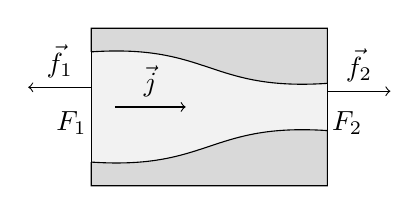
\begin{tikzpicture}
		\draw[fill=black!5!white] (-1.5,-1) rectangle (1.5,1) node[anchor=north east] {$ V $};
		\draw[fill=black!15!white] (-1.5,.7) .. controls (0,.8) and (0,.2) .. (1.5,.3) -- ++(0,.7) -- ++(-3,0) -- ++(0,-.3);
		\draw[fill=black!15!white] (-1.5,-.7) .. controls (0,-.8) and (0,-.2) .. (1.5,-.3) -- ++(0,-.7) -- ++(-3,0) -- ++(0,.3);
		\draw[->] (-1.2,0) -- node[above] {$ \vec{j} $} (-.3,0);
		\node at (-1.75,-.2) {$ F_1 $};
		\draw[->] (-1.5,.25) -- node[above] {$ \vec{f}_1 $} (-2.3,.25);
		\node at (1.75,-.2) {$ F_2 $};
		\draw[->] (1.5,.2) -- node[above] {$ \vec{f}_2 $} (2.3,.2);
	\end{tikzpicture}
\end{minipage}%
\begin{minipage}{.65\linewidth}
	\begin{equation*}
	\prd{}{t} \int_V \dd^3 r \rho(\vec{r},t) = - \int_{\partial V} \dd \vec{f} \cdot \vec{j}(\vec{r},t)
	\end{equation*}
	\begin{equation*}
	\Rightarrow \quad 0 = \ub{\prd{}{t} \int_V \dd ^3 r \rho(\vec{r},t)}_{=\int_V \dd^3 r \prt{\rho}{t}} + \ub{\int_{\partial V} \dd \vec{f} \cdot \vec{j}(\vec{r},t)}_{=\int_V \dd^3 r \vabla \cdot \vec{j}}
	\end{equation*}
	\begin{equation*}
	\Rightarrow \quad \int_V \dd^3 r \left(\prt{\rho}{t} + \vabla \cdot \vec{j}\right) = 0
	\end{equation*}
\end{minipage}%

\noindent
für beliebige $ V $
\frbox{Kontinuitätsgleichung}{
\begin{equation*}
\prt{\rho(\vec{r},t)}{t} + \vabla \cdot \vec{j}(\vec{r},t) = 0
\end{equation*}
}

\subsection{Magnetostatik}

Stationärer (zeitunabhängigen) Fall
$$\underline{\rho = \rho(\vec{r}), \quad \vec{j} = \vec{j}(\vec{r})}$$
$$\prt{}{t}\rho = 0 \quad \Rightarrow \quad \vabla \cdot \underbrace{\vec{j}(\vec{r})}_{\mathclap{\textrm{Stationäre Ströme}}} = 0$$
Konsequenz: Durch jeden Querschnitt eines Leiters fließt der selbe Strom.
$$0 = \int_V \difi{^3 r} \vabla\cdot\vec{j} = \int_{\partial V} \difi{\vec{f}} \cdot \vec{j} = \int_{F_1} \difi{\vec{f}} \cdot \vec{j} + \int_{F_2}\difi{\vec{f}} \cdot \vec{j} = -I_1 + I_2$$
$$\Rightarrow I_1 = I_2$$

% Vorlesung 03.12.18 (21 days until christmas)

\section{Gesetz von Biot-Savart}

stationärer Strom in Leiter $ \rightarrow $ Magnetfeld\\
\begin{minipage}{.7\linewidth}
	Das Magnetfeld $ \dd\vec{B} $ am Ort $ \vec{r} $ verursacht durch Strom $ I $ im Linienelement $ \dd \vec{l} $ in $ \vec{r}' $.
	\begin{equation*}
	\dd \vec{B}(\vec{r}) = k' I \dd \vec{l} \times \frac{\vec{r} - \vec{r}'}{|\vec{r} - \vec{r}'|^3}
	\end{equation*}
	\begin{equation*}
	|\dd \vec{B}| \propto I ,\  |\dd \vec{l}| ,\ \frac{1}{|\vec{r} - \vec{r}'|^2}
	\end{equation*}
	\begin{equation*}
	\tx{Richtung von:} \quad \dd \vec{B} \propto \dd\vec{l} \times (\vec{r},\vec{r}')
	\end{equation*}
\end{minipage}%
\begin{minipage}{.3\linewidth}
	%t1:
	\centering
	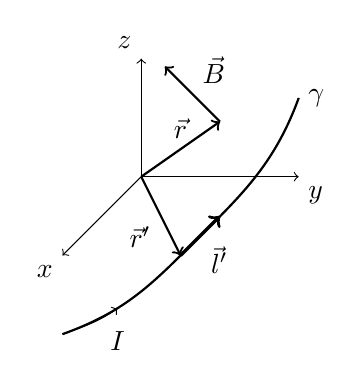
\begin{tikzpicture}
		\draw[->] (0,0) -- (0,1.5) node[anchor=south east] {$ z $};
		\draw[->] (0,0) -- (2,0) node[anchor=north west] {$ y $};
		\draw[->] (0,0) -- (-1,-1) node[anchor=north east] {$ x $};
		\draw[thick, ->] (0,0) -- node[above] {$ \vec{r} $} (1,.7);
		\draw[thick, ->] (1,.7) -- node[anchor=south west] {$ \dd\vec{B} $} ++(-.7,.7);
		\draw[thick, ->] (0,0) -- node[anchor=north east] {$ \vec{r}' $} (.5,-1);
		\draw[very thick, ->] (.5,-1) -- node[anchor=north west] {$ \dd \vec{l}' $} ++(.5,.5);
		\draw[thick] (-1,-2) to[out=20,in=-135] (.5,-1) to[out=45,in=-110] (2,1);
		\draw[->] (-1,-2) to[out=20,in=-145] (-.3,-1.67) node[below=5pt] {$ I $};
		\node[right] at (2,1) {$ \gamma $};
	\end{tikzpicture}
\end{minipage}%
\\
Die Konstante $ k' $ im SI-Einheiten-System ist:
\begin{equation*}
k' = \frac{\mu_0}{4 \pi}
\end{equation*}
$ \mu_0 $ ist die magnetische Feldkonstante, die Permeabilität des Vakuums
\begin{equation*}
\mu_0 = 4 \pi \cdot 10^{-7} \frac{\tx{V s}}{\tx{A m}}
\end{equation*}
Sie ist definiert über:
\begin{equation*}
\epsilon_0 \mu_0 = \frac{1}{c^2} \qquad c: \tx{ Lichtgeschw. in Vakuum}
\end{equation*}
Einheit:
\begin{equation*}
[\vec{B}] = \frac{\tx{V s}}{\tx{m}^2} = 1 \tx{ Tesla}
\end{equation*}\\[5pt]
\frbox{Biot-Savart-Gesetz}{
\begin{equation*}
\vec{B}(\vec{r}) = \frac{\mu_0}{4 \pi} I \int_{\gamma} \dd \vec{l}' \times \frac{\vec{r} - \vec{r}'}{|\vec{r} - \vec{r}'|^3}
\end{equation*}
}
\noindent
Diese Formel gibt das Magnetfeld für einen Stromdurchflossenen dünnen Leiter an.\\[5pt]
Für eine ausgedehnte Stromdichte $ \vec{j}(\vec{r}) $ gilt:
\begin{equation*}
\tx{,,} \dd^3 r \vec{j}(\vec{r}) = I \dd \vec{l}`` \quad \vec{B}(\vec{r}) = \frac{\mu_0}{4 \pi} \int \dd^3 r \vec{j}(\vec{r}') \times \frac{\vec{r}- \vec{r}'}{|\vec{r} - \vec{r}'|^3}
\end{equation*}
Ähnlich in der Elektrostatik:
\begin{equation*}
\vec{E}(\vec{r}) = \frac{1}{4 \pi \epsilon_0} \int \dd^3 r' \rho(\vec{r}') \frac{\vec{r} - \vec{r}'}{|\vec{r} - \vec{r}'|^3}
\end{equation*}
Hier ist $ \rho(\vec{r}) $ aber ein Skalarfeld. $ \vec{j}(\vec{r}) $ ist ein Vektorfeld! Deshalb ist die Berechnung von Magnetfeldern komplizierter.\\[5pt]
\begin{minipage}{.7\linewidth}
	\emph{Beispiel:} Magnetfeld eines langen Drahtes:
	\begin{equation*}
	\vec{j}(\vec{r}) = I \delta(x) \delta(y) \vec{e}_z
	\end{equation*}
	Setzen wir dies nun ins Biot-Savart-Gesetz ein, erhalten wir das $ \vec{B} $-Feld dieses Leiters:
\end{minipage}%
\begin{minipage}{.3\linewidth}
	%t2:
	\centering
	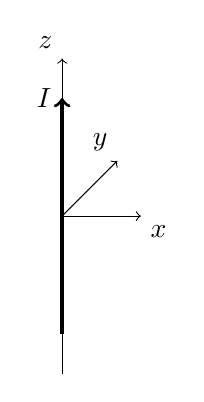
\begin{tikzpicture}
		\draw[very thick, ->] (0,-1.5) -- (0,1.5) node[left] {$ I $};
		\draw[->] (0,-2) -- (0,2) node[anchor=south east] {$ z $};
		\draw[->] (0,0) -- (.7,.7) node[anchor=south east] {$ y $};
		\draw[->] (0,0) -- (1,0) node[anchor=north west] {$ x $};
	\end{tikzpicture}
\end{minipage}%
\\
\begin{align*}
\vec{B}(\vec{r}) \ &= \frac{\mu_0}{4 \pi} \int \dd^3 r' I \delta (x') \delta (y') \vec{e}_z \times \frac{\vec{r} - \vec{r}'}{|\vec{r} - \vec{r}'|^3}\\
&= \frac{\mu_0}{4 \pi} \int_{-\infty}^{\infty} \dd z' \vec{e}_z \times \frac{\vec{r} - \equaltoup{\vec{r}'}{\mathclap{\vec{r}' = (0,0,z')}}}{|\vec{r} - \vec{r}'|^3}\\
\end{align*}
Nebenrechnung:\\
$ \vec{B}(\vec{r}) $ hängt nicht von $ z $ ab $ \rightarrow \vec{r} = (x,y,0) \quad \rightarrow \vec{r} - \vec{r}' = (x,y,-z') $\\
$ \vec{e}_z \times (\vec{r} - \vec{r}') = \begin{pmatrix}
-y \\ x \\ 0
\end{pmatrix} $
\begin{align*}
\qquad \qquad &= \frac{\mu_0 I}{4 \pi} \begin{pmatrix}
-y \\ x \\ 0
\end{pmatrix} \int_{-\infty}^{\infty} \dd z' \frac{1}{[x^2 + y^2 + z'^2]^{3/2}} \tag{*} \label{integral}\\
&= \frac{\mu_0 I}{4 \pi} \frac{2}{x^2 + y^2} \begin{pmatrix}
-y \\ x \\ 0
\end{pmatrix}\\
\vec{B} (\vec{r}) &= \frac{\mu_0 I}{2 \pi} \frac{1}{x^2 + y^2} \begin{pmatrix}
-y \\ x \\ 0
\end{pmatrix}
\end{align*}
In Zylinderkoordinaten:
\begin{equation*}
\vec{r} = \begin{pmatrix}
\rho \cos \varphi \\ \rho \sin \varphi \\ z
\end{pmatrix} \qquad \rho^2 = x^2 + y^2
\end{equation*}
\begin{equation*}
\vec{e}_{\varphi} = \frac{\prt{\vec{r}}{\varphi}}{|\prt{\vec{r}}{\varphi}|} = \frac{1}{\rho} \begin{pmatrix}
- \rho \sin \varphi \\ \rho \cos \varphi \\ 0
\end{pmatrix} = \frac{1}{\sqrt{x^2 + y^2}} \begin{pmatrix}
-y \\ x \\ 0
\end{pmatrix}
\end{equation*}
\begin{minipage}{.5\linewidth}
	\begin{equation*}
	\Rightarrow \quad \vec{B} = \frac{\mu_0}{2 \pi} I \frac{1}{\rho} \vec{e}_{\varphi}
	\end{equation*}
\end{minipage}%
\begin{minipage}{.5\linewidth}
	\centering
	%t3:
	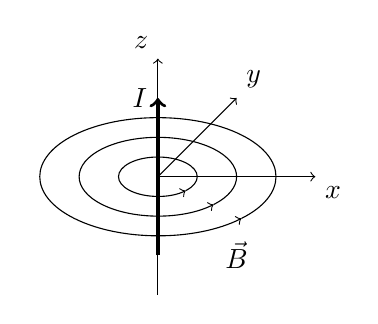
\begin{tikzpicture}
		\draw[->] (0,-1.5) -- (0,1.5) node[anchor=south east] {$ z $};
		\draw[very thick, ->] (0,-1) -- (0,1) node[left] {$ I $};
		\draw[->] (0,0) -- (2,0) node[anchor=north west] {$ x $};
		\draw[->] (0,0) -- (1,1) node[anchor=south west] {$ y $};
		\draw[->] ({.5 * sin(45)},-{.25 * cos(45)}) arc[start angle=-45,end angle=315, x radius=.5, y radius=.25];
		\draw[->] ({1 * sin(45)},-{.5 * cos(45)}) arc[start angle=-45, end angle=315, x radius=1, y radius=.5];
		\draw[->] ({1.5 * sin(45)}, -{.75 * cos(45)}) arc[start angle=-45, end angle=315, x radius=1.5, y radius=.75];
		\node at (1,-1) {$ \vec{B} $};
	\end{tikzpicture}
\end{minipage}%

\section{Kraft eines äußeren Magnetfeldes auf einen Stromdurchflossenen Leiter}

\begin{minipage}{.5\linewidth}
	%t4:
	\centering
	\begin{tikzpicture}
		\draw[->] (0,0) -- (0,1.5) node[anchor=south east] {$ z $};
		\draw[->] (0,0) -- (2.5,0) node[anchor=north west] {$ x $};
		\draw[->] (0,0) -- (-1,-1) node[anchor=north east] {$ y $};
		\foreach \y in {.4,1.2,-.4,-1.2,-2}
		\draw[->] (.5,\y) -- ++(1.5,0);
		\node[right] at (2,1.2) {$ \vec{B} $};
		\coordinate (o) at (1,-1);
		\draw[thick, ->] (-1,-.5) to[out=-30,in=180] (o) to[out=0,in=-150] (3,-.5) to[out=30,in=-120] (3.5,0) node[anchor=north west] {$ I $};
		\draw[blue,thick, ->] ($ (o) + (.5,0.02) $) -- node[left] {$ \dd \vec{F} $} ++(0,.5);
		\draw[red,thick, ->] ($ (o) + (.5,0.02) $) -- node[below,xshift=10pt] {$ \dd \vec{l} $} ++(1,.1);
	\end{tikzpicture}
\end{minipage}%
\begin{minipage}{.5\linewidth}
	\begin{equation*}
	\dd \vec{F} = I \dd \vec{l} \times \vec{B}(\vec{r})
	\end{equation*}
	\begin{equation*}
	|\dd\vec{F}| \propto I ,\ |\dd \vec{l}| ,\ |\vec{B}|
	\end{equation*}
	\begin{equation*}
	\tx{Richtung von:} \quad \dd \vec{F} \propto \dd \vec{l} \times \vec{B}(\vec{r})
	\end{equation*}
\end{minipage}%
\\
\begin{minipage}{.6\linewidth}
	Damit ist die Kraft auf eine beliebige Leiterschleife:
	\begin{equation*} % \gamma_2 ?
	\vec{F} = I \int_{\gamma} \dd \vec{l} \times \vec{B}(\vec{r})
	\end{equation*}
\end{minipage}%
\begin{minipage}{.4\linewidth}
	\centering
	%t5:
	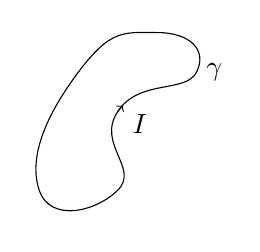
\begin{tikzpicture}
		\draw plot [smooth cycle, tension=1] coordinates { (0,0) (1,.5) (.5,1) (-.5,.5) (-1,-1) (0,-1) };
		\draw[->] (0,0) -- ++(50:.1cm) node[anchor=north west] {$ I $};
		\node[right] at (1,.5) {$ \gamma $};
	\end{tikzpicture}
\end{minipage}%
\\
Für eine ausgedehnte Stromverteilung gilt dann:
\begin{equation*}
\vec{F} = \int \dd ^3 r \ \vec{j}(\vec{r}) \times \vec{B}(\vec{r})
\end{equation*}

\subsection{Kraft zwischen zwei Stromdurchflossenen Leitern}

$ I_2 $ erzeugt am Ort $ \vec{r}_1 $ das Magnetfeld:
\begin{equation*}
\vec{B}(\vec{r}_1)  = \frac{\mu_0}{4 \pi} I_2 \int_{\gamma} \dd \vec{l}_2 \times \frac{\vec{r}_1 - \vec{r}_2}{|\vec{r}_1 - \vec{r}_2|^3}
\end{equation*}
\begin{minipage}{.6\linewidth}
	$ \rightarrow $ Kraft auf Linienelement $ \dd \vec{l}_1 $ in $  \vec{r}_1 $:
	\begin{align*}
	\dd \vec{F}_{12} &= I_1 \dd \vec{l}_1 \times \vec{B}(\vec{r}_1)\\
	&= \frac{\mu_0}{4 \pi} I_1 I_2 \dd \vec{l}_1 \times \int_{\gamma_{2}} \times \frac{\vec{r}_1 - \vec{r}_2}{|\vec{r}_1 - \vec{r}_2|^3}
	\end{align*}
	%
	%
	% ich glaube hier fehlt was dl_2 im integral
	%
	%
\end{minipage}%
\begin{minipage}{.4\linewidth}
	\flushright
	%t6:
	\begin{tikzpicture}
		\draw plot [smooth cycle, tension=.9] coordinates { (0,0) (-1,0) (-1,-1) (-1.3,-1.7) (-1,-2) (-.3,-1.5) (0,-.8)  };
		\draw[shift={(2 cm, -2 cm)},rotate=200] plot [smooth cycle, tension=.9] coordinates { (0,0) (-1,0) (-1,-1) (-1,-2) (-.3,-1.5) (0,-.8)  };
		\coordinate (o) at (1,-2.5);
		\coordinate (l) at (-.3,-1.5);
		\coordinate (r) at ($ (o) + (.75,1)$);
		\draw[thick,->] (o) -- node[above] {$ \vec{r}_1 $} (l);
		\draw[thick,->] (o) -- node[above,xshift=-5pt] {$ \vec{r}_2 $} (r);
		\node[anchor=north west] at (o) {$ O $};
		\draw[red,thick,->] (l) -- node[left,yshift=5pt] {$ \dd \vec{l}_1 $} ++(50:.5cm);
		\draw[red,thick,->] (r) -- node[right] {$ \dd \vec{l}_2 $} ++(95:.5cm);
		\draw[->] (-.2,.11) -- ++(160:.1cm) node[anchor=south west] {$ I_1 $};
		\node at (-1.2,.2) {$ \gamma_1 $};
		\draw[->] (2.415,0) -- ++(105:.1cm) node[anchor=south west] {$ I_2 $};
		\node at (1.5,-.3) {$ \gamma_2 $};
	\end{tikzpicture}
\end{minipage}%
\\
Die Kraft auf Leiterschleife 1 ist dann:
\begin{equation*}
\vec{F}_{12} = \frac{\mu_0}{4 \pi} I_1 I_2 \int_{\gamma_1} \int_{\gamma_2} \dd \vec{l}_1 \times \left(\dd \vec{l}_2 \times \frac{\vec{r}_1 - \vec{r}_2}{|\vec{r}_1 - \vec{r}_2|^3}\right)
\end{equation*}
\emph{Beispiel:} \textbf{Kraft zwischen zwei parallelen Drähten}\\
\begin{minipage}{.6\linewidth}
	\begin{equation*}
	\dd \vec{F}_{12} = \frac{\mu_0}{4 \pi} I_1 I2 \equalto{\dd \vec{l}_1}{\vec{e}_z \dd l_1} \times \int_{\gamma} \dd \vec{l}_2 \times \frac{\vec{r}_1 - \vec{r}_2}{|\vec{r}_1 - \vec{r}_2|^3}
	\end{equation*}
	Aus der Skizze gilt:\\
	$ \dd \vec{l}_2 = \dd z_2 \vec{e}_z \qquad \vec{r}_1  = (0,0,0) \qquad \vec{r}_2 = (a,0,z_2) $
\end{minipage}%
\begin{minipage}{.4\linewidth}
	\flushright
	%t7:
	\begin{tikzpicture}[scale=1.2]
		\draw[->] (0,-1) -- (0,2) node[anchor=south east] {$ z $};
		\draw[->] (-.5,0) -- (3,0) node[anchor=north west] {$ x $};
		\draw (2,-1) -- (2,2);
		\draw[thick,->] (0,-.5) -- (0,1.5) node[left] {$ I_1 $};
		\draw[thick,->] (2,-.5) -- (2,1.5) node[right] {$ I_2 $};
		\coordinate (o) at (0,0);
		\coordinate (p) at (2,.5);
		\draw[decorate, decoration={brace,amplitude=10pt,mirror,raise=2pt}]
		(o) -- node[below=12pt] {$ a $} (2,0);
		\draw[thick,->] (o) -- node[above] {$ \vec{r}_{2} $} (p);
		\draw[red,thick,->] (o) -- node[left] {$ \dd \vec{l}_1 $} ($ (o) + (0,.5) $);
		\draw[red,thick,->] (p) -- node[right] {$ \dd \vec{l}_2 $} ($ (p) + (0,.5) $);
	\end{tikzpicture}
	\vspace{5pt}
\end{minipage}%
\\
Nebenrechnung:
\begin{equation*}
\dd \vec{l}_2 \times (\vec{r}_1 - \vec{r}_2) = \dd z_2 \begin{pmatrix}
0 \\ 0 \\ 1
\end{pmatrix} \times \begin{pmatrix}
-a \\ 0 \\ -z_2
\end{pmatrix} = \dd z_2 \begin{pmatrix}
0 \\ -a \\ 0
\end{pmatrix}
\end{equation*}
\vspace{5pt}

\noindent
\begin{minipage}{.75\linewidth}
	\begin{align*}
	\rightarrow \quad \dd \vec{F}_{12} = \frac{\mu_0}{4 \pi} I_1 I_2 \dd l_1 \ub{\vec{e}_z \times \begin{pmatrix}
		0 \\ -a \\ 0
		\end{pmatrix}}_{= a \vec{e}_x} \ub{\int_{-\infty}^{\infty} \dd z_2 \frac{1}{\left(a^2 + z_2^2\right)^{3/2}}}_{\mathclap{\quad \qquad \qquad = \frac{2}{a^2} \ \ \tx{wie oben} (\ref{integral})}}
	\end{align*}
\end{minipage}%
\begin{minipage}{.25\linewidth}
	Richtung:\\
	\flushright
	%t8:
	\begin{tikzpicture}
	\draw[->] (0,0) -- (0,1);
	\draw[->] (1,0) -- (1,1);
	\draw[->] (0,.5) -- (.3,.5);
	\draw[->] (1,.5) -- (.7,.5);
	%2nd
	\coordinate (o) at (2.5,0);
	\draw[->] (o) -- ++(0,1);
	\draw[->] ($ (o) + (1,1)$) -- ++(0,-1);
	\draw[->] ($ (o) + (0,.5)$) -- ++(-.3,0);
	\draw[->] ($ (o) + (1,.5)$) -- ++(.3,0);
	\end{tikzpicture}
\end{minipage}%
\begin{center}
	\begin{minipage}{.5\linewidth}
		\frbox{Kraft pro Länge:}{
			\begin{equation*}
			\frac{\dd \vec{F}_{12}}{\dd l_1} = \frac{\mu_0}{2 \pi} \frac{I_1 I_2}{a} \vec{e}_x
			\end{equation*}}
	\end{minipage}
\end{center}

\section{Feldgleichungen der Magnetostatik und Vektorpotential}

\begin{equation*}
\vec{B}(\vec{r}) = \frac{\mu_0}{4 \pi} \int \dd^3 r' \vec{j}(\vec{r}') \times \frac{\vec{r} - \vec{r}'}{|\vec{r} - \vec{r}'|^3}
\end{equation*}

\subsection{Vektorpotential}

\begin{equation*}
\vec{B}(\vec{r}) = \frac{\mu_0}{4 \pi} \int \dd^3 r' \ub{\vec{j}(\vec{r'}) \times \ub{\frac{\vec{r} - \vec{r}'}{|\vec{r} - \vec{r}'|^3}}_{- \vabla_{\vec{r}} \frac{1}{|\vec{r} - \vec{r}'|}}}_{\vabla_{\vec{r}} \times \left(\vec{j}(\vec{r'}) \frac{1}{|\vec{r} - \vec{r}'|}\right)}
\end{equation*}
Mit einer Identität des ersten Übungsblattes:
\begin{equation*}
\vabla \times (f \vec{G}) = f \vabla \times \vec{G} - \vec{G} \times \vabla f
\end{equation*}
(Die Rotation von $ \vec{G} $ fällt weg, da $ \vec{j} $ nur von $ \vec{r}' $ abhängt.)
\begin{equation*}
\Rightarrow \quad \vec{B}(\vec{r}) = \vabla_{\vec{r}} \times \frac{\mu_0}{4 \pi} \int \dd^3 r'\frac{\vec{j}(\vec{r}')}{|\vec{r} - \vec{r}'|} = \vabla \times \custo{\rightarrow}{\vec{A}(\vec{r})}{\mathclap{\tx{Vektorpotential}}}
\end{equation*}
\begin{equation*}
\vec{B}(\vec{r}) = \vabla \times \vec{A}(\vec{r}) \quad \leftarrow \vec{A} \tx{ nicht eindeutig festgelegt}
\end{equation*}
\begin{align*}
& \vec{A}' = \vec{A} + \vec{G} \ \tx{ mit } \ \vabla \times \vec{G} = 0 \quad \rightarrow \quad \vec{G}(\vec{r}) = \vabla \Lambda (\vec{r})\\
& \rightarrow \quad \vabla \times \vec{A}' = \vabla \times \vec{A} + \vabla \times \vec{G} = \vec{B}
\end{align*}
\begin{equation*}
\Rightarrow \quad \vec{A}(\vec{r}) = \frac{\mu_0}{4 \pi} \int \dd^3 r' \frac{\vec{j}(\vec{r}')}{|\vec{r} - \vec{r}'|} + \vabla \Lambda (\vec{r}) \quad \Rightarrow \quad \vabla \times \vec{A}(\vec{r}) = \vec{B}(\vec{r})
\end{equation*}
\textbf{Transformation: Eichtransformation}
\begin{equation*}
\vec{A}(\vec{r}) \rightarrow \vec{A}' = \vec{A} + \vabla \Lambda
\end{equation*}
\textbf{Magnetostatik: übliche Wahl:} $ \Lambda \equiv 0 $
\begin{equation*}
\Rightarrow \quad \vec{A} = \frac{\mu_0}{4 \pi} \int \dd ^3 r' \frac{\vec{j}(\vec{r}')}{|\vec{r} - \vec{r}'|}
\end{equation*}
Eine andere Eichung ist die \textbf{Coulomb-Eichung:}
\begin{equation*}
\Rightarrow \quad \vabla \cdot \vec{A} = 0
\end{equation*}
\begin{align*}
\vabla \cdot \vec{A} &= \frac{\mu_0}{4 \pi} \int \dd^3 r' \ub{\vabla_{\vec{r}} \cdot \left(\vec{j}(\vec{r}') \frac{1}{|\vec{r} - \vec{r}'|}\right)}\\
& \qquad \qquad \qquad = \vec{j}(\vec{r}') \cdot \ub{\vabla_{\vec{r}} \frac{1}{|\vec{r} - \vec{r}'|}}_{-\vabla_{\vec{r}'} \frac{1}{|\vec{r} - \vec{r}'|}}\\
& \qquad \qquad \qquad = - \vabla_{\vec{r}'} \cdot \left(\vec{j}(\vec{r}') \frac{1}{|\vec{r} - \vec{r}'|}\right) + \ob{\left(\vabla_{\vec{r}'} \cdot \vec{j}(\vec{r}')\right)}^{=0} \frac{1}{|\vec{r} - \vec{r}'|}\\
&= - \frac{\mu_0}{4 \pi} \int_{\mathbb{R}^3} \dd^3 r' \vabla_{\vec{r}'} \cdot \left(\frac{\vec{j}(\vec{r}')}{|\vec{r} - \vec{r}'|}\right)\\
&= - \frac{\mu_0}{4 \pi} \lim\limits_{R \to \infty} \int\limits_{K_R(0)} \dd^3 r' \vabla_{\vec{r}'} \cdot \left(\frac{\vec{j}(\vec{r}')}{|\vec{r} - \vec{r}'|}\right)\\
&= \frac{\mu_0}{4 \pi} \ub{\lim\limits_{R\to \infty} \int\limits_{\partial K_R(0)} \dd \vec{f}' \cdot \frac{\vec{j} (\vec{r}')}{|\vec{r} - \vec{r}'|}}_{=0} = 0
\end{align*}
\emph{Beispiel:} \textbf{homogenes Magnetfeld}
\begin{equation*}
\vec{B} = \vec{B}_0 \qquad \vec{B} = \vabla \times \vec{A}
\end{equation*}
\begin{equation*}
\vec{A} = \frac{1}{2} \vec{B} \times \vec{r}
\end{equation*}
Mit der Identität:
\begin{equation*}
\vabla \times (\vec{a} \times \vec{b}) = \vec{a} (\vabla \cdot \vec{b}) - \vec{b} (\vabla \cdot \vec{a}) + (\vec{b} \cdot \vabla) \vec{a} - (\vec{a} \cdot \vabla) \vec{b}
\end{equation*}
\begin{equation*}
\rightarrow \quad \vabla \times \vec{A} = \frac{1}{2} \vabla \times (\vec{B} \times \vec{r}) = \frac{1}{2} \vec{B} \ub{\vabla \cdot \vec{r}}_{= 3} - \frac{1}{2} \ub{(\vec{B} \cdot \vabla) \vec{r}}_{= \vec{B}} = \vec{B}
\end{equation*}
%
%
%
% I32 N soll wahrscheinlich B sein + weiter unten fehlt 1/2
%
%
%
Mit der Identität:
\begin{equation*}
\vabla \cdot (\vec{a} \times \vec{b}) = \vec{b} \cdot (\vabla \times \vec{a}) - \vec{a} \cdot (\vabla \times \vec{b})
\end{equation*}
\begin{equation*}
\Rightarrow \quad \vabla \cdot \vec{A} = \frac{1}{2} \vabla \cdot \left(\vec{B} \times \vec{r}\right) = - \frac{1}{2} \vec{B} \cdot \ub{\left(\vabla \times \vec{r}\right)}_{= 0} = 0
\end{equation*}
andere mögliche Wahl:
\begin{equation*}
\vec{A}' = \frac{1}{2} \vec{B} \times \vec{r} + \ub{\vabla \frac{r^2}{2}}_{=\vec{r}} = \vec{A} + \vec{r}
\end{equation*}
\begin{equation*}
\vabla \times \vec{A}' = \ub{\vabla \times \vec{A}}_{= \vec{B}} + \ub{\vabla \times \vec{r}}_{= 0} = \vec{B}
\end{equation*}

% Vorlesung 6.12.18 (18 days until christmas)

\begin{equation*}
\rmbox{\vec{B}(\vec{r}) = \frac{\mu_0}{4 \pi} \int \dd ^3 r' \vec{j}(\vec{r}') \times \frac{\vec{r} - \vec{r}'}{|\vec{r} - \vec{r}'|^3} = \vabla \times \vec{A}(\vec{r})}
\end{equation*}

\subsection{Feldgleichungen der Magnetostatik}

\subsubsection{Divergenz (Quellen)}

\begin{equation*}
\vabla \cdot \vec{B}(\vec{r}) = \vabla \cdot (\vabla \times \vec{A}(\vec{r})) = 0
\end{equation*}
\begin{equation*}
\rmbox{\Rightarrow \quad \vabla \cdot \vec{B}(\vec{r}) = 0}
\end{equation*}
In der Elektrostatik gilt:
\begin{equation*}
\rmbox{\vabla \cdot \vec{E}(\vec{r}) = \frac{1}{\epsilon_0} \rho(\vec{r})}
\end{equation*}
Es gibt also keine ,,magnetischen Ladungen`` wie beim elektrischen Feld.\\[5pt]
integrale Formulierung:
\begin{equation*}
0 = \int_V \dd^3 r \vabla \cdot \vec{B} = \int_{\partial V} \dd \vec{f} \cdot \vec{B}
\end{equation*}

\subsubsection{Rotation (Wirbel)}

$ \vec{B} = \vec{\nabla} \times \vec{A} $
\begin{equation*}
\vec{A}(\vec{r}) = \frac{\mu_0}{4 \pi} \int \dd^3 r' \frac{\vec{j}(\vec{r}')}{|\vec{r} - \vec{r}'|} + \vabla \Lambda
\end{equation*}
\begin{align*}
\Rightarrow \quad \vabla \times \vec{B} &= \vabla \times (\vabla \times \vec{A})\\
&= \vabla (\vabla \cdot \vec{A}) - \Delta \vec{A}
\end{align*}
\begin{equation*}
\vabla \cdot \vec{A} = \ub{\vabla \cdot \left(\frac{\mu_0}{4 \pi} \int \dd ^3 r' \frac{\vec{j}(\vec{r}')}{|\vec{r} - \vec{r}'|}\right)}_{=0} + \vabla \cdot (\vabla \Lambda) = \Delta \Lambda 
\end{equation*}
\begin{equation*}
\Delta \vec{A} = \frac{\mu_0}{4 \pi} \int \dd^3 r' \vec{j}(\vec{r}') \ub{\Delta \frac{1}{|\vec{r} - \vec{r}'|}}_{= - 4 \pi \delta(\vec{r} - \vec{r}')} + \Delta \vabla \Lambda = - \mu_0 \vec{j}(\vec{r}) + \Delta (\vabla \Lambda)
\end{equation*}
mit: $ \Delta \vec{A} = \begin{pmatrix}
\Delta A_x \\ \Delta A_y \\ \Delta A_z
\end{pmatrix} $
\begin{equation*}
\Rightarrow \quad \vabla \times \vec{B} = \cancel{\vabla(\Delta \Lambda)} + \mu_0 \vec{j} - \cancel{\Delta (\vabla \Lambda)} = \mu_0 \vec{j}
\end{equation*}
Kürzbar, da partielle Ableitungen vertauschbar sind.
\begin{equation*}
\rmbox{\vabla \times \vec{B} = \mu_0 \vec{j}}
\end{equation*}
\begin{minipage}{.8\linewidth}
	integrale Formulierung:
	\begin{equation*}
	\int_{\partial F} \dd \vec{r} \cdot \vec{B} (\vec{r}) = \int_F \dd \vec{f} \cdot (\vec{\nabla} \times \vec{B}) = \mu_0 \ub{\int_F \dd \vec{f} \cdot \vec{j}(\vec{r})}_{I_F} = \mu_0 I_F
	\end{equation*}
\end{minipage}%
\begin{minipage}{.2\linewidth}
	%t1:
	\flushright
	\begin{tikzpicture}
		\draw[->,pattern=north east lines, pattern color=black!40!white] (1,0) arc[start angle=0,end angle=360,y radius=.5cm,x radius=1cm] node[right] {$ \partial F $};
		\node at (-.6,0) {$ F $};
		\draw[fill=white] (-.25,1.5) -- (-.25,0) arc[start angle=180,end angle=360,x radius=.25,y radius=.125] -- (.25,1.5);
		\draw (0,1.5) ellipse (.25cm and .125cm);
		\draw (-.25,-1)  arc[start angle=180,end angle=360,x radius=.25,y radius=.125];
		\draw (-.25,-1) -- (-.25,-.48);
		\draw (.25,-1) -- (.25,-.48);
		\node at (0,.75) {$ \vec{j} $};
	\end{tikzpicture}
\end{minipage}%
\\[5pt]
\frbox{Amp\`eresches Durchflutungsgesetz}{
\begin{equation*}
\Rightarrow \quad \oint_{\partial F} \dd \vec{r}\cdot \vec{B}(\vec{r}) = \mu_0 I_F
\end{equation*}
}

\subsubsection{Magnetfeld eines stromdurchflossenen Leiters mit homogener Stromdichte}

\begin{minipage}{.7\linewidth}
	Aufgrund der Symmetrie verwenden wir Zylinderkoordinaten:
	\begin{equation*}
	\vec{r} = \begin{pmatrix}
	\rho \cos \varphi \\ \rho \sin \varphi \\ z
	\end{pmatrix}
	\end{equation*}
	Die Stromdichte ist dann:
	\begin{align*}
	\vec{j} &= \vec{e}_z \casess{\frac{I}{\pi R^2}}{\rho \le R}{0}{\tx{sonst.}}\\
	&= \vec{e}_z \frac{I}{\pi R^2} \theta(R - \rho)
	\end{align*}
	Symmetrie:
	\begin{equation*}
	\vec{B}(\vec{r}) = B_\varphi(\rho) \vec{e}_{\varphi} \qquad \vec{e}_{\varphi} = \begin{pmatrix}
	- \sin \varphi \\ \cos \varphi \\ 0
	\end{pmatrix}
	\end{equation*}
\end{minipage}%
\begin{minipage}{.3\linewidth}
	%t2:
	\flushright
	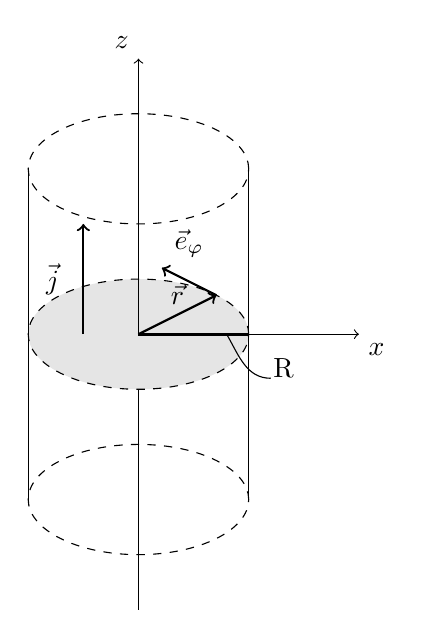
\begin{tikzpicture}[scale=1.4]
		\draw[dashed,fill=gray!20!white] (0,0) ellipse (1cm and .5cm);
		\draw[dashed] (0,-1.5) ellipse (1cm and .5cm);
		\draw[dashed] (0,1.5) ellipse (1cm and .5cm);
		\draw[->] (0,0) -- (0,2.5) node[anchor=south east] {$ z $};
		\draw (0,-.5) -- (0,-2.5);
		\draw[->] (0,0) -- (2,0) node[anchor=north west] {$ x $};
		\draw (-1,-1.5) -- (-1,1.5) (1,-1.5) -- (1,1.5);
		\draw[thick,->] (-.5,0) -- node[left=5pt] {$ \vec{j} $} (-.5,1);
		\draw[very thick] (0,0) -- (1,0) node[anchor=north west,xshift=5pt,yshift=-5pt] {R};
		\draw[thick,->] (0,0) -- node[above] {$ \vec{r} $} ({cos(45) * 1cm},{sin(45) * .5cm});
		\draw[thick,->] ({cos(45) * 1cm},{sin(45) * .5cm}) -- node[above=5pt] {$ \vec{e}_\varphi $} ++({-cos(45) * .7cm},{sin(45) * .35cm});
		\draw (.8,0) to[out=-60,in=180] (1.2,-.4);
	\end{tikzpicture}
\end{minipage}%

\noindent
\begin{minipage}{.6\linewidth}
	$ F $ ist ein Kreis mit Radius $ \rho $ (kleiner oder größer als $ R $)\\
	Hierauf wenden wir das Amp\`eresche Durchflutungsgesetz an:\\
	Unter Verwendung von:
	\begin{equation*}
	\dd \vec{f}' = \vec{e}_z \dd f = \vec{e}_z \rho' \dd \rho' \dd \varphi'
	\end{equation*}
\end{minipage}%
\begin{minipage}{.4\linewidth}
	%t3:
	\flushright
	\begin{tikzpicture}[scale=.8]
		\draw[->] (-3,0) -- (3,0) node[anchor=north west] {$ x $};
		\draw[->] (0,-3) -- (0,3) node[anchor=south east] {$ y $};
		\draw[dashed] (0,0) circle (2cm);
		\draw[draw=none,pattern=north east lines, pattern color=black!30!white] (0,0) circle (2cm);
		\draw (0,0) circle (1cm);
		\node at (1,-1) {$ R $};
		\draw[thick,->] (0,0) -- node[above=5pt] {$ \vec{r} $} ({sin(60) * 2cm},{cos(60) * 2cm});
		\draw (-1.2,1.2) to[out=90,in=0] (-2,2) node[left] {$ F $};
	\end{tikzpicture}
\end{minipage}%
\\
\begin{align*}
\mu_0 \int_F \dd \vec{f} ' \cdot \vec{j}(\vec{r}') &= \int_{\partial F} \dd \vec{r}' \cdot \vec{B}(\vec{r}')\\
&= \mu_0 \int_{0}^{\rho} \dd\rho' \int_{0}^{2 \pi} \dd \varphi'\rho' \frac{I}{\pi R^2} \theta(R - \rho)\\
&= \mu_0 \frac{I}{\pi R^2} 2 \pi \ub{\int_{0}^{\rho} \dd \rho' \rho' \theta(R - \rho)}\\
& \qquad = \left\{\begin{array}{cc}
\int_{0}^{R} \dots = \frac{1}{2} R^2 & \rho > R \\[5pt]
\int_{0}^{\rho}\: \dots = \frac{1}{2} \rho^2 & \rho \le R
\end{array}\right.
\end{align*}
\begin{equation*}
\Rightarrow \quad \mu_0 \int_{F} \dd \vec{f}' \cdot \vec{j}(\vec{r}') = \mu_0 \casess{I}{\rho > R}{\frac{\rho^2}{R^2} I}{\rho \le R}
\end{equation*}
\begin{equation*}
\int_{\partial F}\dd \vec{r}' \cdot \vec{B}(\vec{r}') = \int_{0}^{2 \pi} \dd \varphi \frac{\dd \vec{r}'}{\dd \varphi} \cdot \vec{B} = \int_{0}^{2 \pi} \dd \varphi \rho B_{\varphi}(\rho) = 2 \pi \rho B_{\varphi}(\rho)
\end{equation*}
mit:
\begin{equation*}
\vec{r}(\rho) = \begin{pmatrix}
\rho \cos \varphi \\ \rho \sin \varphi \\ 0
\end{pmatrix} \qquad \frac{\dd r'}{\dd \varphi} = \begin{pmatrix}
- \rho \sin \varphi \\ \rho \cos \varphi \\ 0
\end{pmatrix} = \rho \vec{e}_{\varphi}
\end{equation*}
Damit erhalten wir:
\begin{equation*}
 \mu_0 \int_{F} \dd \vec{f}' \cdot \vec{j}(\vec{r}')  = 2 \pi \rho B_{\varphi}(\rho) 
\end{equation*}
Daraus folgt:
\begin{equation*}
\Rightarrow \quad \mu_0 I_F = \rho B_{\varphi}(\rho) 2 \pi
\end{equation*}
Dies können wir umstellen in:
\begin{equation*}
\Rightarrow \quad B_{\varphi} (\rho) = \frac{\mu_0}{2 \pi} \frac{I_F}{\rho}
\end{equation*}
\begin{equation*}
\Rightarrow \quad \vec{B}(\vec{r}) = \frac{\mu_0}{2 \pi} I \vec{e}_{\varphi} \casess{\frac{1}{\rho}}{\rho > R}{\frac{\rho}{R^2}}{\rho \le R}
\end{equation*}
\begin{minipage}{.5\linewidth}
	%t4:
	\centering
	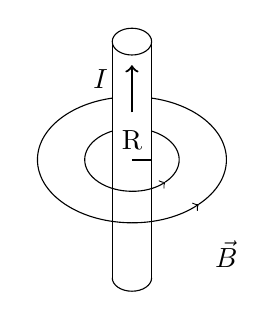
\begin{tikzpicture}
		\draw[->] ({sin(45) * .6cm},{- cos(45) * .4cm}) arc[start angle=-45,end angle=315,x radius = .6cm,y radius=.4cm];
		\draw[->] ({sin(45) * 1.2cm},{- cos(45) * .8cm}) arc[start angle=-45,end angle=315,x radius = 1.2cm,y radius=.8cm];
		\draw[draw=none,fill=white] (-.25,0) rectangle (.25,1.5);
		\draw (-.25,-1.5) -- (-.25,1.5) (.25,-1.5) -- (.25,1.5);
		\draw[thick] node[above] {R}  (0,0) -- (.25,0);
		\node at (1.2,-1.2) {$ \vec{B} $};
		\draw[->,thick] (0,.6) -- (0,1.2) node[left=5pt,yshift=-5pt] {$ I $};
		\draw (0,1.5) ellipse (.25cm and .17cm);
		\draw (-.25,-1.5) arc[start angle=180,end angle=360, x radius=.25, y radius=.17];
	\end{tikzpicture}
\end{minipage}%
\begin{minipage}{.5\linewidth}
	\vspace{15pt}
	%t5:
	\centering
	\begin{tikzpicture}
		\draw[thick,->] (0,0) -- (0,3) node[anchor=south east] {$ B_\varphi (\rho) $};
		\draw[thick,->] (0,0) -- (4,0) node[anchor=north west] {$ \rho $};
		\draw (2,.1) -- (2,-.1) node[below] {R};
		\draw (0,0) -- (2,2) to[out=-75,in=170] (4,.25);
		\draw (.1,2) -- (-.1,2) node[left] {$ \frac{\mu_0}{2 \pi} I \frac{1}{R} $};
		\draw[dashed] (0,2) -| (2,0);
	\end{tikzpicture}
\end{minipage}%


\subsubsection{Differentialgleichung für das Vektorpotential}

\begin{equation*}
\vec{B} = \vabla \times \vec{A} \qquad \vabla \times \vec{B} = \mu_0 \vec{j}
\end{equation*}
\begin{align*}
\mu_0 \vec{j} &= \vabla \times \vec{B} = \vabla \times (\vabla \times \vec{A})\\
&= \vabla(\vabla \cdot \vec{A}) - \Delta \vec{A}
\end{align*}
falls $ \vabla\cdot \vec{A} = 0 $ (Coulomb-Eichung)  % (Coulomb-Gleichung)
\begin{equation*}
\Rightarrow \quad \rmbox{\Delta \vec{A} = -\mu_0 \vec{j}}
\end{equation*}
Wichtig: Die Komponenten sind nicht unabhängig voneinander aufgrund unserer Annahme $ \vabla \cdot \vec{A} = 0 $
analog:$ \Delta \Phi = - \frac{1}{\epsilon_0} \rho $

\subsection{Feldgleichungen der Magnetostatik \texorpdfstring{\tiny(Wiederholung)}{Wiederholung}}

\begin{minipage}{.5\linewidth}
	\begin{equation*}
	\vabla \cdot \vec{B} = 0 \ \ 
	\end{equation*}
	\vspace{-5pt}
	\begin{equation*}
	\phantom{\quad (\tx{Amp\`ere})} \vabla \times \vec{B} = \mu_0 \vec{j} \quad (\tx{Amp\`ere})
	\end{equation*}
\end{minipage}%
\begin{minipage}{.5\linewidth}
	\begin{equation*}
	\int_{\partial V} \dd \vec{f} \cdot \vec{B} = 0 \quad \ \ \, \,
	\end{equation*}
	\begin{equation*}
	\int_{\partial F} \dd \vec{r} \cdot \vec{B} = \mu_0 I_F
	\end{equation*}
\end{minipage}%
\\
Und für das Vektorpotential:
\begin{equation*}
\vec{B} = \vabla \times \vec{A} \qquad \Rightarrow \Delta  \vec{A} = - \mu_0 \vec{j}
\end{equation*}

\section{Multipolentwicklung - Magnetisches Moment}

\begin{equation*}
\vec{A}(\vec{r}) = \frac{\mu_0}{4 \pi} \int \dd ^3 r' \frac{\vec{j}(\vec{r}')}{|\vec{r} - \vec{r}'|}
\end{equation*}
mit $ \vabla \cdot \vec{A} = 0 $ (Coulomb-Eichung)\\
\begin{minipage}{.5\linewidth}
	Wir betrachten eine lokalisierte Ladungsverteilung:
	\begin{equation*}
	\vec{j}(\vec{r}) = \casess{\tx{beliebig}}{r < R}{0}{r > R}
	\end{equation*}
\end{minipage}%
\begin{minipage}{.5\linewidth}
	%t6:
	\flushright
	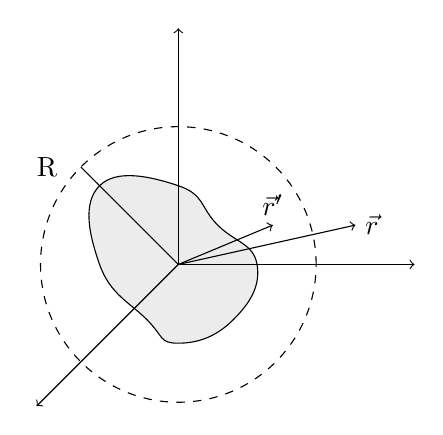
\begin{tikzpicture}
		\draw[fill=gray!15!white]  plot [smooth cycle, tension=0.8] coordinates { (-1,0) (-1,1) (0,1) (.5,.5) (1,0) (.7,-.7) (0,-1) (-.4,-.7) };
		\draw[->] (0,0) -- (0,3);
		\draw[->] (0,0) -- (3,0);
		\draw[->] (0,0) -- (-1.8,-1.8);
		\draw[dashed] (0,0) circle (1.75cm);
		\draw (0,0) -- ({- sin(45) * 1.75},{cos(45) * 1.75})node[left=5pt] {R};
		\draw[->] (0,0) -- (1.2,.5) node[above] {$ \vec{r}' $};
		\draw[->] (0,0) -- (2.25,.5) node[right] {$ \vec{r} $};
	\end{tikzpicture}
\end{minipage}%
\\
Für $ r > R > r' $ machen wir eine Taylorentwicklung:
\begin{equation*}
\frac{1}{|\vec{r} - \vec{r}'|} = \frac{1}{r} + \frac{\vec{r}}{r^3} \cdot \vec{r}' + \dots
\end{equation*}
\begin{equation*}
\Rightarrow \quad \vec{A}(\vec{r}) = \frac{\mu_0}{4 \pi} \left\{\frac{1}{r} \int \dd^3r' \vec{j} (\vec{r}') + \frac{1}{r^3} \int \dd ^3 r' (\vec{r} \cdot \vec{r}') \vec{j}(\vec{r}') + \dots \right\}
\end{equation*}
\textbf{Es gilt: in der Magnetostatik} $ \vabla \cdot \vec{j} = 0 $
\begin{enumerate}[i)]
	\item Das Integral über die Stromdichte verschwindet:\\
	\begin{minipage}{.5\linewidth}
		$$ \int \dd ^3 r' \vec{j} (\vec{r}') = 0 $$
	\end{minipage}%
	\begin{minipage}{.5\linewidth}
		%t7:
		\centering
		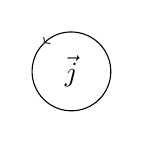
\begin{tikzpicture}[scale=.5]
			\draw[->] (0,0) arc[start angle=135, end angle=495, radius = 1];
			\node at ({sin(45)},{-cos(45)}) {$ \vec{j} $};
		\end{tikzpicture}
	\end{minipage}%
	\\
	\item $$ \int \dd^3 r' (\vec{r} \cdot \vec{r}') \vec{j}(\vec{r}) = - \vec{r} \times \ub{\frac{1}{2} \int \dd^3 r' (\vec{r}' \times \vec{j}(\vec{r}'))}_{\mathclap{\substack{\defeq \vec{m}\\ \tx{magnetisches} \\ \tx{Dipolmoment} }}} $$
\end{enumerate}
Die Entwicklung des Vektorpotentials wird dann zu:
\begin{equation*}
\Rightarrow \quad \vec{A}(\vec{r}) = \frac{\mu_0}{4 \pi} \ub{\frac{\vec{m} \times \vec{r}}{r^3}}_{\propto \frac{1}{r^2}}
\end{equation*}
Für das Magnetfeld gilt:
\begin{equation*}
\Rightarrow \quad \vec{B} = \vabla \times \vec{A} = \frac{\mu_0}{4 \pi} \vabla \times \left(\vec{m} \times \frac{\vec{r}}{r^3}\right)
\end{equation*}
Mit der Identität: $ \vabla \times (f \vec{G}) = f \vabla \times \vec{G} - \vec{G} \times \vabla f $
\begin{align*}
\vabla \times \left(\frac{1}{r^3} (\vec{m} \times \vec{r})\right) &= \frac{1}{r^3} \ub{\vabla \times (\vec{m} \times \vec{r})}_{= 2 \vec{m}} - (\vec{m} \times \vec{r}) \times \ub{\vabla \frac{1}{r^3}}_{= - \frac{3 \vec{r}}{r^5}}\\
&= \frac{1}{r^3} 2 \vec{m} + \frac{3}{r^5} \ub{(\vec{m} \times \vec{r}) \times \vec{r}}_{(\vec{m} \cdot \vec{r}) \vec{r} - (\vec{r} \cdot \vec{r}) \vec{m}}\\
&= \frac{3 \vec{r} (\vec{m} \vec{r})}{r^5} - \frac{\vec{m}}{r^3}
\end{align*}
Beim $ \vec{B} $-Feld erhalten wir für den ersten nicht verschwindenden Term den Dipolterm:\\
\frbox{Multipolentwicklung des Magnetfeldes (1. Term)}{
	\begin{equation*}
	\Rightarrow \quad \vec{B}(\vec{r}) = \frac{\mu_0}{4 \pi} \left[\frac{3 \vec{r}(\vec{m} \cdot \vec{r})}{r^5} - \frac{\vec{m}}{r^3}\right] \qquad r > R
	\end{equation*}
}

\noindent
Der große Unterschied zum $ \vec{E} $-Feld ist, dass der führende Term ein Dipol ist. Das $ \vec{B} $-Feld hat also keinen Monopol.\\[5pt]
\emph{Beispiel:} \textbf{Magnetisches Dipolmoment einer Drahtschleife}\\
\begin{minipage}{.5\linewidth}
	$$ \rho = \sqrt{x^2 + y^2} \qquad \vec{e}_{\varphi} = \begin{pmatrix}
	- \sin \varphi \\ \cos \varphi \\ 0
	\end{pmatrix}$$
\end{minipage}%
\begin{minipage}{.5\linewidth}
	%t8:
	\centering
	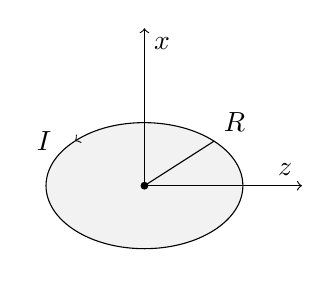
\begin{tikzpicture}
		\draw[->,fill=gray!10!white] ({-sin(45) * 1.25},{cos(45) * .8}) arc[start angle=135, end angle=495, x radius = 1.25, y radius = .8] node[left=5pt] {$ I $};
		\draw[->] (0,0) -- (0,2) node[anchor=north west] {$ x $};
		\draw[->] (0,0) -- (2,0) node[anchor=south east] {$ z $};
		\node[circle,fill=black,inner sep=1pt,minimum size=1pt] at (0,0) {};
		\draw (0,0) -- ({sin(45) * 1.25},{cos(45) * .8}) node[anchor=south west] {$ R $};
	\end{tikzpicture}
\end{minipage}%
\\
\begin{equation*}
\vec{j} = I \delta(\rho - R) \delta(z) \vec{e}_{\varphi}
\end{equation*}
\begin{equation*}
\vec{m} = \frac{1}{2} \int \dd^3 r \ \vec{r} \times \vec{j}(\vec{r})
\end{equation*}
Nebenrechnung:
\begin{align*}
\vec{r} \times \vec{e}_{\varphi} &= \begin{pmatrix}
\rho \cos \varphi \\ \rho \sin \varphi \\ z
\end{pmatrix} \times \begin{pmatrix}
- \sin \varphi \\ \cos \varphi \\ ß
\end{pmatrix}\\
&= \begin{pmatrix}
- z \cos \varphi \\ - z \sin \varphi \\ \rho
\end{pmatrix}\\
&= \rho \begin{pmatrix}
0 \\ 0 \\ 1
\end{pmatrix} - z \begin{pmatrix}
\cos \varphi \\ \sin \varphi \\ 0
\end{pmatrix}\\
&= \rho \vec{e}_z - z \vec{e}_{\varphi}
\end{align*}
\begin{align*}
\Rightarrow \quad \vec{m} &= \frac{1}{2} I \int_{0}^{\infty} \rho \ \dd \rho \int_{0}^{2 \pi} \dd \varphi \int_{-\infty}^{\infty} \dd z \ \delta(\rho - R) \delta(z) (\rho \vec{e}_z - \custo{\rightarrow}{z}{0} \vec{e}_{\varphi})\\
&= \frac{I}{2} R^2 2 \pi \vec{e}_z
\end{align*}
\begin{minipage}{.5\linewidth}
	\begin{equation*}
	\Rightarrow \quad \vec{m} = \ub{\pi R^2}_{F} I \vec{e}_z = F I \vec{e}_z
	\end{equation*}
\end{minipage}%
\begin{minipage}{.5\linewidth}
	%t9:
	\centering
	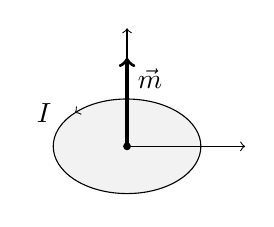
\begin{tikzpicture}[scale=.75]
		\draw[->,fill=gray!10!white] ({-sin(45) * 1.25},{cos(45) * .8}) arc[start angle=135, end angle=495, x radius = 1.25, y radius = .8] node[left=5pt] {$ I $};
		\draw[->] (0,0) -- (0,2);
		\draw[->] (0,0) -- (2,0);
		\node[circle,fill=black,inner sep=1pt,minimum size=1pt] at (0,0) {};
		\draw[very thick,->] (0,0) -- (0,1.5) node[anchor=north west] {$ \vec{m} $};
	\end{tikzpicture}
	\vspace{5pt}
\end{minipage}%
\\
\begin{minipage}{.5\linewidth}
	Das Magnetische Moment einer Spule:
	\begin{equation*}
	\vec{m} = N I \cdot F \vec{e}_z
	\end{equation*}
\end{minipage}%
\begin{minipage}{.5\linewidth}
	%t10:
	\centering
	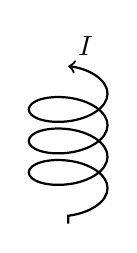
\begin{tikzpicture}
		\draw[decorate,decoration={aspect=.5, segment length=4mm, amplitude=.5cm,coil},thick,<-] (0,2) node[anchor=south west] {$ I $} -- (0,0);
	\end{tikzpicture}
	\vspace{10pt}
\end{minipage}%
\\
\folie{Vergleich idealer Dipol und Leiterschleife}\\
\folie{Vergleich $ \vec{E} $-Feld einer elektrischer Dipol und Magnetfeld um Leiterschleife}

% Vorlesung 10.12.18 (14 Days until christmas)

\subsection{Kraft auf eine lokalisierte Stromverteilung in einem äußeren Magnetfeld \texorpdfstring{$ \vec{B} $}{B}}

\begin{minipage}{.6\linewidth}
	$ \vec{j}(\vec{r}) = 0 \ \tx{ für } \ |\vec{r}| > 0 $
	Taylorentwicklung von $ \vec{B}(\vec{r}) $ um $ \vec{r} = 0 $:
	\begin{equation*}
	\vec{B}(\vec{r}) = \vec{B}(0) + (\vec{r} \cdot \vabla) \vec{B}(\vec{r}) \bigg|_{\vec{r} = 0} + \dots
	\end{equation*}
	\begin{equation*}
	\longrightarrow \quad \vec{F} = \int \dd^3 r \left(\vec{j}(\vec{r}) \times \vec{B} (\vec{r})\right) \quad \ \
	\end{equation*}
\end{minipage}%
\begin{minipage}{.4\linewidth}
	%t1:
	\flushright
	\begin{tikzpicture}
		\draw[fill=gray!10] plot [smooth cycle, tension=.8] coordinates { (.5,-1.5) (0,-1) (-.7,-.5) (-.7,.7) (.7,1) (.7,0) (1.2,-.7) };
		\draw[->] (0,0) -- (0,2) node[anchor=south east] {$ z $};
		\draw[->] (0,0) -- (2,0) node[anchor=north west] {$ x $};
		\draw[->] (0,0) -- (-1.4,-1.4) node[anchor=north east] {$ y $};
		\node at (-.3,.45) {$ \vec{j} $};
		\coordinate (a) at (1.5,1.7);
		\coordinate (b) at ($ (a) + (-44:.5) $);
		\coordinate (c) at ($ (a) + (-45:1) $);
		\coordinate (d) at ($ (a) + (-50:1.5) $);
		\draw[<-] (a) to[out=-150,in=10] ++(-160:4);
		\draw[<-] (b) to[out=-145,in=15] ++(-155:4.5);
		\draw[<-] (c) to[out=-145,in=35] ++(-145:4.5);
		\draw[<-] (d) to[out=-145,in=55] ++(-135:4);
		\node at (2.5,1.5) {$ \vec{B} $};
		\draw[dashed] (0,0) circle (1.7cm);
	\end{tikzpicture}
\end{minipage}%
\begin{equation*}
\vec{F} = \ub{\int\dd^3 r \left(\vec{j}(\vec{r}) \times \vec{B}(0)\right)}_{= \bigg(\ub{\int \dd^3 r \vec{j} (\vec{r})}_{= 0} \bigg) \times \vec{B}(0)} + \int\dd ^3 r \left[ \vec{j}(\vec{r}) \times (\vec{r} \cdot \vabla) \vec{B}(\vec{r}) \right] + \dots
\end{equation*}
\begin{minipage}{.7\linewidth}
	Der verschwindende Teil ist ein homogenes $ \vec{B} $-Feld ($ \vec{B} = \const $), und übt daher keine Kraft auf Stromverteilung aus.
\end{minipage}%
\begin{minipage}{.3\linewidth}
	%t2:
	\flushright
	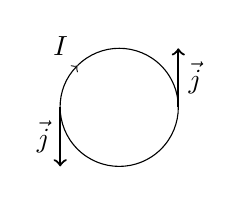
\begin{tikzpicture}[scale=.75]
		\draw[->] (-{sin(45) * 1},{cos(45) * 1}) arc[start angle=135,end angle=-225, radius=1cm] node[anchor=south east] {$ I $};
		\draw[thick,->] (-1,0) -- node[left] {$ \vec{j} $} ++(0,-1);
		\draw[thick,->] (1,0) -- node[right] {$ \vec{j} $} ++(0,1);
	\end{tikzpicture}
\end{minipage}%
\\
Die Komponenten des Kraftvektors sind:
\begin{equation*}
\vec{F}_i = \int \dd^3 r \left[\vec{j} \times (\vec{r} \cdot \vabla) \vec{B}\right]_i
\end{equation*}
Nun nutzen wie die folgende Identität:
\begin{equation*}
(\vec{a} \times \vec{b})_i = \sum_{k,l} \epsilon_{ikl} \ a_k b_l
\end{equation*}
$ \epsilon_{ikl} $ ist das Levi-Civita Symbol.\\
Damit ergibt sich:
\begin{align*}
\left(\vec{j} \times (\vec{r} \cdot \vabla) \vec{B}\right)_i &= \sum_{k,l} \epsilon_{ikl} \  j_k \ub{\left[(\vec{r} \cdot \vabla) \vec{B}\right]_l}_{(\vec{r} \cdot \vabla) B_l = (\vabla B_l) \cdot \vec{r}}\\
&= \sum_{k,l} \epsilon_{ikl} \ j_k (\vabla B_l \cdot \vec{r})
\end{align*}
\begin{align*}
\rightarrow \quad F_i &= \sum_{k,l} \epsilon_{ikl} \ \ub{\int \dd ^3 r \left[(\vabla B_l) \cdot \vec{r}\right] j_k}\\
&\qquad \qquad = \int \dd^3 r \left( \left[(\vabla B_l) \cdot \vec{r}\right] \vec{j}\right)_k \overset{\tx{Identität}}{=} - \frac{1}{2} \left[\vabla B_l \times \int \dd^3 r \ \vec{r} \times \vec{j} \right]
\end{align*}
Hier die benutzte Identität (aus den Hausaufgaben):
\begin{equation*}
\frac{1}{2} \vec{a} \times \int \dd ^3 r (\vec{r} \times \vec{j} (\vec{r})) = - \int \dd^3 r (\vec{a} \cdot \vec{r}) \vec{j}(\vec{r}) \qquad (\vabla \cdot \vec{j} = 0)
\end{equation*}
Damit ergibt sich für die Kraft:
\begin{align*}
F_i &= - \frac{1}{2} \sum_{k,l} \epsilon_{ikl} \ \Bigg[\vabla B_l \times \ub{\int \dd^3 r \ \vec{r} \times \vec{j}(\vec{r})}_{=2 \vec{m}}\Bigg]_k \\
&= - \sum_{k,l} \epsilon_{ikl} \ \ub{\left(\vabla B_l \times \vec{m}\right)}_{\mathclap{ \qquad \qquad - \left[\vec{m} \times \vabla B_l\right]_k = - (\vec{m} \times \vabla)_k B_l}}\\
&= \sum_{k,l} \epsilon_{ikl} \ (\vec{m} \times \vabla)_k B_l\\
&= \left[(\vec{m} \times \vabla) \times \vec{B}\right]_i
\end{align*}
\begin{equation*}
\rmbox{F_i = \left[(\vec{m} \times \vabla) \times \vec{B}\right]_i}
\end{equation*}
Wir können nun mit der Identität umschreiben:
\begin{equation*}
(\vec{a} \times \vec{b}) \times \vec{c} = \vec{b} (\vec{c} \cdot \vec{a}) - \vec{a} (\vec{b} \cdot \vec{c})
\end{equation*}
\begin{align*}
\vec{F} &= (\vec{m} \times \vabla) \times \vec{B}(0)\\
&= \vabla (\vec{m} \cdot \vec{B}) - \vec{m} (\ub{\vabla \cdot \vec{B}}_{=0})
\end{align*}
\begin{equation*}
\rmbox{\Rightarrow \quad \vec{F} = \vabla (\vec{m} \cdot \vec{B}(0))}
\end{equation*}
Also: $ \vec{m} \perp \vec{B} \Rightarrow \vec{F} = 0 $\\
\begin{minipage}{.5\linewidth}
	\textbf{$ \rightarrow $ potentielle Energie:}
	\begin{equation*}
	W = - \vec{m} \cdot \vec{B}(0)
	\end{equation*}
\end{minipage}%
\begin{minipage}{.5\linewidth}
	%t3:
	\centering
	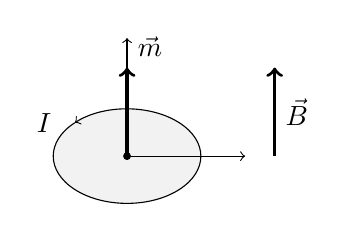
\begin{tikzpicture}[scale=.75]
		\draw[->,fill=gray!10!white] ({-sin(45) * 1.25},{cos(45) * .8}) arc[start angle=135, end angle=495, x radius = 1.25, y radius = .8] node[left=5pt] {$ I $};
		\draw[->] (0,0) -- (0,2);
		\draw[->] (0,0) -- (2,0);
		\node[circle,fill=black,inner sep=1pt,minimum size=1pt] at (0,0) {};
		\draw[very thick,->] (0,0) -- (0,1.5) node[anchor=south west] {$ \vec{m} $};
		\draw[very thick,->] (2.5,0) -- node[right] {$ \vec{B} $} ++(0,1.5);
	\end{tikzpicture}
\end{minipage}%
\\
\textbf{Drehmoment:}
\begin{equation*}
\vec{N} = \vec{m} \times \vec{B}(0)
\end{equation*}
\begin{equation*}
\vec{N} = \int\dd^3 r \ \vec{r} \times (\vec{j} \times \vec{B})
\end{equation*}

\section{Magnetostatik in Materie}

mikroskopische Feldgleichungen:
\begin{equation*}
\vabla \cdot \vec{B} = 0 \qquad \vabla \times \vec{B} = \mu_0 \vec{j}
\end{equation*}

\subsection{Makroskopische Feldgleichungen}

Definition Mittlung:
\begin{equation*}
\langle \vec{B} \rangle (\vec{r}) = \int\dd^3r' f(\vec{r}') \vec{B}(\vec{r} - \vec{r}')
\end{equation*}
Es muss weiterhin gelten:
\begin{equation*}
\vabla \cdot \langle \vec{B} \rangle (\vec{r}) = 0 \qquad \vabla \times \langle \vec{B} \rangle (\vec{r}) = \mu_0 \langle \vec{j} \rangle (\vec{r})
\end{equation*}
\lcom{Aus Zeitgründen werden wir hier nichts weiter genau herleiten wie in der Elektrostatik, sondern im wesentlichen die Ergebnisse Besprechen.}\\[5pt]
Aufteilung der Stromdichte:
\begin{equation*}
\vec{j} = \vec{j}_g + \vec{j}_f
\end{equation*}
$ \langle j_g \rangle $\\
\begin{minipage}{.5\linewidth}
	\centering
	%t4:
	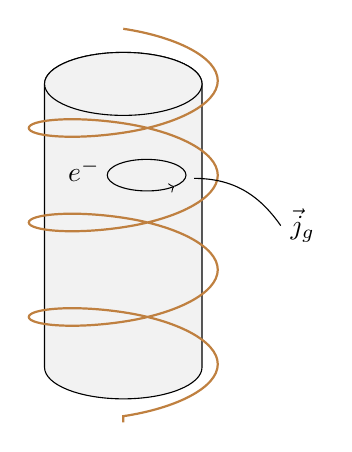
\begin{tikzpicture}
		\draw[fill=gray!10!white] (-1,1.8) -- (-1,-1.8) arc[start angle=180,end angle=360,x radius=1cm,y radius=.4cm] (1,-1.8) -- (1,1.8) arc[start angle=0,end angle=180,x radius=1cm,y radius=.4cm];
		\draw[fill=gray!10!white] (0,1.8) ellipse (1cm and .4cm);
		\draw[decorate,decoration={coil,aspect=.3,amplitude=12mm,segment length=12mm},brown,thick] (0,2.5) -- (0,-2.5);
		\node at (-.5,.7) {$ e^- $};
		\draw[->] (.65,.5) arc[start angle=-45,end angle=315,x radius=.5,y radius=.2];
		\draw (.9,.6) to[out=0,in=125] (2,0) node[right] {$ \vec{j}_g $};
	\end{tikzpicture}
\end{minipage}%
\begin{minipage}{.5\linewidth}
	\centering
	%t5:
	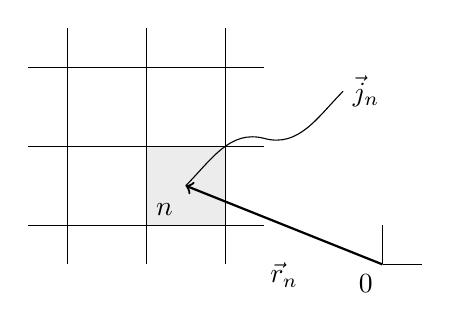
\begin{tikzpicture}
	\draw[draw=none,fill=gray!15!white] (1.5,.5) rectangle ++(1,1);
	\foreach \x in {.5,1.5,2.5}
	\draw (\x,0) -- (\x,3);
	\foreach \y in {.5,1.5,2.5}
	\draw (0,\y) -- (3,\y);
	\coordinate (o) at (4.5,0);
	\draw (o) -- ++(0,.5);
	\draw (o) -- ++(.5,0);
	\draw[thick,->] (o) -- node[below=10pt] {$ \vec{r}_n $} (2,1);
	\node[anchor=south west] at (1.5,.5) {$ n $};
	\draw (2,1) to[out=45,in=165] ++(1,.6) to[out=-15,in=-135] ++(1,.6) node[right] {$ \vec{j}_n $};
	\node[anchor=north east] at (o) {$ 0 $};
	\end{tikzpicture}
\end{minipage}%
\\
Mittlung:
\begin{align*}
\rightarrow \quad \langle \vec{j}_g \rangle &= \vabla \times \ub{\langle \sum_n \vec{m} \delta(\vec{r}' - \vec{r}_n) \rangle}_{\defeq \vec{M}(\vec{r})} (\vec{r}) + \dots \\
&= \vabla \times \vec{M}(\vec{r})
\end{align*}
Mit
$$ \vec{m}_n = \frac{1}{2} \int \dd^3 r' \vec{r}' \times \vec{j}_n(\vec{r}') $$
Und $ \vec{M} (\vec{r}) : $ makroskopische Magnetisierung
\begin{equation*}
\left[\vec{M}\right] = \frac{\tx{A}}{\tx{m}^2} \tx{m} = \frac{\tx{A}}{\tx{m}} = \frac{\tx{magnetisches Dipolmoment}}{\tx{Volumen}}
\end{equation*}
\begin{equation*}
\Rightarrow \quad \vabla \times \langle \vec{B} \rangle (\vec{r}) = \mu_0 \langle \vec{j} \rangle (\vec{r}) = \mu_0 \langle \vec{j}_f \rangle (\vec{r}) + \mu_0 \vabla \times \vec{M}(\vec{r}) + \dots
\end{equation*}
\begin{equation*}
\Rightarrow \quad \vabla \times \ub{\left(\frac{1}{\mu_0} \langle \vec{B} \rangle (\vec{r})  - \vec{M} (\vec{r}) - \dots \right)}_{\defeq \vec{H}(\vec{r})} = \langle \vec{j}_f \rangle (\vec{r})
\end{equation*}
\begin{equation*}
\left[\vec{H}\right] = \frac{\tx{A}}{\tx{m}}
\end{equation*}

\subsection{Makroskopische Feldgleichunge der Magnetostatik}

\begin{equation*}
\vabla \cdot \vec{B} = 0 \qquad \vabla \times \vec{H} = \vec{j}_f \qquad 
\end{equation*}
\begin{equation*}
\vec{H} = \frac{1}{\mu_0} \vec{B} - \vec{M} - \dots
\end{equation*}
Integrale Form:
\begin{equation*}
\oint_{\partial V} \dd \vec{f} \cdot \vec{B} = \int_V \dd^3 r \vabla \cdot \vec{B} = 0
\end{equation*}
\begin{equation*}
\oint_{\partial F} \dd \vec{r} \cdot \vec{H} = \int_{F} \dd \vec{f} \vabla \times \vec{H} = \int_{F} \dd \vec{f} \cdot \vec{j}_f = I_F
\end{equation*}
\begin{center}
	%t6:
	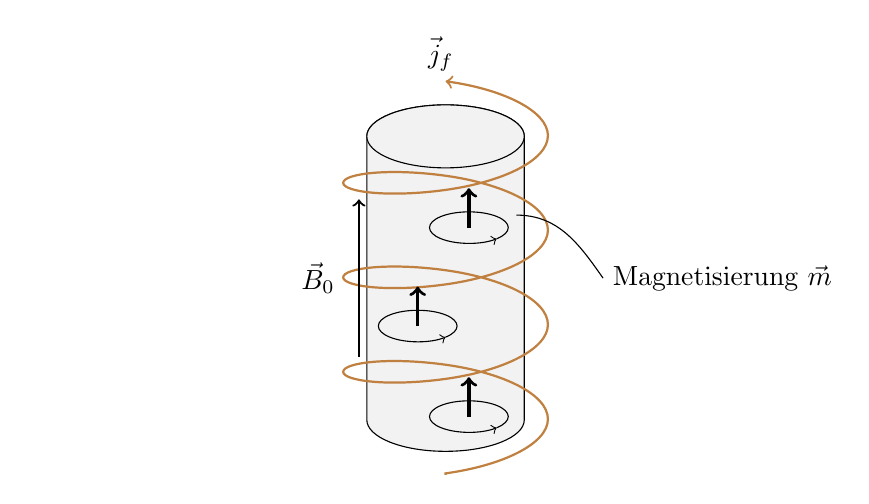
\begin{tikzpicture}
		\draw[fill=gray!10!white] (-1,1.8) -- (-1,-1.8) arc[start angle=180,end angle=360,x radius=1cm,y radius=.4cm] (1,-1.8) -- (1,1.8) arc[start angle=0,end angle=180,x radius=1cm,y radius=.4cm];
		\draw[fill=gray!10!white] (0,1.8) ellipse (1cm and .4cm);
		\draw[decorate,decoration={coil,aspect=.3,amplitude=13mm,segment length=12mm},<-,brown,thick] (0,2.5) node[above] {\color{black} $ \vec{j}_f $ \color{brown}} -- (0,-2.5);
		
		\foreach \x\y\c in {.65/.5/1,0/-.75/2,.65/-1.9/3}
		\coordinate (\c) at ({\x - sin(45) * .5}, {\y + cos(45) * .2});
		
		\foreach \x\y in {.65/.5,0/-.75,.65/-1.9}
		\draw[->] (\x,\y) arc[start angle=-45,end angle=315,x radius=.5,y radius=.2];
		
		\foreach \c in {1,2,3}
		\draw[very thick,->] (\c) -- ++(0,.5);
		
		\draw (.9,.8) to[out=0,in=125] (2,0) node[right] {Magnetisierung $ \vec{m} $};
		\draw[thick,->] (-1.1,-1) -- node[left=5pt] {$ \vec{B}_0 $} ++(0,2);
		
		% ugly alignment line
		\draw[white] (-2,0) -- (-5.3,0);
	\end{tikzpicture}
\end{center}
Magnetisierung $ \rightarrow $ Zusatzfeld $ \vec{B}_M $
\begin{equation*}
\vec{B} = \vec{B}_0 + \vec{B}_M
\end{equation*}
mit $ \vec{B}_0 = \mu_0 \vec{H} $ und $ \vec{B}_M = \mu_0 \vec{M} $

\subsection{Vektorpotential}

\begin{equation*}
\vec{B} = \vabla \times \vec{A} \quad \rightarrow \quad \langle \vec{B} \rangle = \vabla \times \langle \vec{A} \rangle
\end{equation*}
\begin{equation*}
\vec{A} (\vec{r}) = \frac{\mu_0}{4 \pi} \int \dd ^3 r' \frac{\vec{j}(\vec{r}')}{|\vec{r} - \vec{r}'|} \qquad (\Lambda = 0 \quad \vabla \cdot \vec{A} = 0)
\end{equation*}
Wir benutzen $ \langle \vec{j} \rangle = \langle \vec{j}_f \rangle + \langle \vec{j}_g \rangle $ und $ \langle \vec{j}_g \rangle = \vabla \times \vec{M}(\vec{r}) $
\begin{align*}
\Rightarrow \quad \langle \vec{A} \rangle (\vec{r}) &= \frac{\mu_0}{4 \pi} \int \dd^3r' \frac{\langle \vec{j} \rangle (\vec{r}')}{|\vec{r} - \vec{r}'|}\\
&= \frac{\mu_0}{4 \pi} \int \dd^3 r' \frac{\langle \vec{j}_f \rangle (\vec{r}')}{|\vec{r} - \vec{r}'|} + \ub{\frac{\mu_0}{4 \pi} \int\dd^3 r ' \frac{\vabla_{\vec{r}'} \times \vec{M} (\vec{r}')}{|\vec{r} - \vec{r}'|}}\\
& \qquad \qquad \qquad \qquad \quad = \frac{\mu_0}{4 \pi} \int \dd^3 r' \vec{M}(\vec{r}') \times \frac{(\vec{r} - \vec{r}')}{|\vec{r} - \vec{r}'|^3}
\end{align*}
Erklärung der letzten Umformung:
\begin{align*}
\int \dd^3 r' \frac{1}{|\vec{r} - \vec{r}'|} \vabla_{\vec{r}'} \times \vec{M} (\vec{r}') &= \int \dd^3 r' \vabla_{\vec{r}'} \times \left(\frac{1}{|\vec{r} - \vec{r}'|} \vec{M}\right) \ub{- \left(\vabla_{\vec{r}'} \frac{1}{|\vec{r} - \vec{r}'|}\right)}_{= \frac{\vec{r} - \vec{r}'}{|\vec{r} - \vec{r}'|^3}} \times \vec{M}\\
&= \ub{\int\dd^3 r' \vabla_{\vec{r}'} \times \left(\frac{\vec{M}}{|\vec{r} - \vec{r}'|}\right)} + \int\dd^3r' \vec{M}(\vec{r}')  \times \frac{\vec{r} - \vec{r}'}{|\vec{r} - \vec{r}'|^3}\\
&= \lim\limits_{R \to \infty} \int_{K_R(0)} \dd^3 r' \vabla_{\vec{r}'} \times \left(\frac{\vec{M}}{|\vec{r} - \vec{r}'|}\right)\\
&= \int_{\partial K_{R(0)}} \dd \vec{f}' \times \frac{\vec{M}}{|\vec{r} - \vec{r}'|} = 0
\end{align*}

\subsection{Magnetisierung und Suszeptibilität}

\begin{equation*}
\vec{M} = \vec{M}(\vec{H})
\end{equation*}
lineare Näherung, isotrope Medien:
\begin{equation*}
\vec{M} = \chi_m \vec{H}
\end{equation*}
$ \chi_m : $ magnetische Suszeptibilität
\begin{align*}
\rightarrow \quad \vec{B} &= \mu_0 (\vec{H} + \vec{M}) = \mu_0 (\vec{H} + \chi_m \vec{H})\\
&= \ub{(1 + \chi_m)}_{= \mu_r} \mu_0 \vec{H}\\
&= \mu \vec{H}
\end{align*}
$ \mu_r : $ relative Permeabilität\\
$ \mu = \mu_0 \mu_r : $ Permeabilität